%
% anwendungen.tex -- Anwendungen des Skalarproduktes
%
% (c) 2018 Prof Dr Andreas Müller, Hochschule Rapperswil
%
\section{Erste Anwendungen des Skalarproduktes\label{section:normalform}}
\rhead{Erste Anwendungen des Skalarproduktes}
Aus den Eigenschaften des Skalarproduktes ergeben sich unmittelbar
erste Anwendungen.

%
% Normalenform von Ebene und Gerade
%
\subsection{Normalenform von Ebene und Gerade}
\begin{figure}
\begin{center}
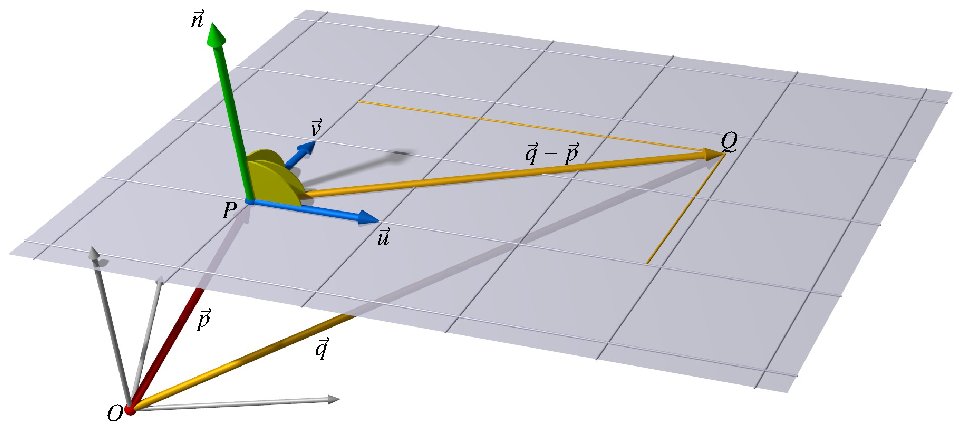
\includegraphics{4/images/normalenform.pdf}
\end{center}
\caption{Ebene in Normalenform\label{image-normalenform}}
\end{figure}
Das Skalarprodukt gibt uns eine neue Möglichkeit, Ebenen zu
beschreiben.
Eine Ebene durch den Punkt $P$ senkrecht auf den Vektor
$\vec n$ besteht genau aus jenen Punkten $Q$, für die der Vektor
$\overset{\rightarrow}{PQ}$ auf $\vec n$ senkrecht steht
(Abbildung~\ref{image-normalenform}).
Mit dem Skalarprodukt
ausgedrückt: Die Menge der Ortsvektoren der Punkte einer Ebene durch $P$ mit
\index{Normale}
Normale $\vec n$ ist
\[
\{\vec r\;|\;(\vec r-\vec p)\cdot \vec n=0\}
\]
Multipliziert man die Gleichung aus, erhält man
\begin{align*}
\left(
\begin{pmatrix}x\\y\\z\end{pmatrix}
-\begin{pmatrix}p_1\\p_2\\p_3\end{pmatrix}\right)\cdot
\begin{pmatrix}n_1\\n_2\\n_3\end{pmatrix}&=0
\\
(x-p_1)n_1+(y-p_2)n_2+(z-p_3)n_3&=0
\\
n_1x+n_2y+n_3z&=p_1n_1+p_2n_2+p_3n_3
\end{align*}
Diese Form der Ebenengleichung, in der $\vec n$ ein Einheitsnormalenvektor ist,
heisst auch {\em Hessesche Normalform}.
\index{Normalenform}
\index{Hessesche Normalform}

\begin{satz}
Ist $\vec n$ ein Einheitsvektor, dann ist
\[
d=(\vec r-\vec p_0)\cdot \vec n
\]
der Abstand des Punktes mit dem Ortsvektor $\vec r$ von der Ebene durch
den Punkt mit Ortsvektor $\vec p_0$ und Normalen $\vec n$.
In Koordinaten:
\[
d=n_xx+n_yy+n_zz-\vec p_0\cdot\vec n
\]
\end{satz}
\begin{proof}[Beweis]
$(\vec r-\vec p)\cdot \vec n$ ist die Länge der Projektion des Vektors
$\vec r -\vec p$ auf den Normalenvektor $\vec n$, also genau der behauptete
Abstand.
\end{proof}

\begin{beispiel}
Man finde die Normalenform der Ebenengleichung (\ref{beispielebene}) auf
Seite~\pageref{beispielebene},
und berechne den Abstand des Punktes $(1,1,1)$ von der Ebene.

\medskip

{\parindent 0pt Die} Lösung vollzieht sich in folgenden Schritten:
\begin{compactenum}
\item Bestimme die Normale der Ebene.
\item Schreibe die Gleichung der Ebene in Normalenform.
\item Bringe die Normalenform in Hessesche Normalform.
\item Berechne den Abstand des Punktes $(1,1,1)$.
\end{compactenum}
Gesucht ist ein Vektor $\vec n$, der auf beiden
Richtungsvektoren senkrecht steht, also
\begin{equation}
\begin{pmatrix}n_1\\n_2\\n_3\end{pmatrix}
\cdot
\begin{pmatrix}2\\2\\-2\end{pmatrix}
=0,
\qquad
\begin{pmatrix}n_1\\n_2\\n_3\end{pmatrix}
\cdot
\begin{pmatrix}3\\-3\\-1\end{pmatrix}
=0
\label{gleichungen-fuer-normale}
\end{equation}
Dies ist gleichbedeutend mit dem Gleichungssystem
\[
\begin{pmatrix}
2&2&-2\\
3&-3&-1
\end{pmatrix}
\begin{pmatrix}n_1\\n_2\\n_3\end{pmatrix}
=\begin{pmatrix}0\\0 \end{pmatrix}
\]
Der Gauss-Algorithmus liefert
\begin{align*}
\begin{tabular}{|>{$}c<{$}>{$}c<{$}>{$}c<{$}|}
\hline
2%
\begin{picture}(0,0)
\color{red}\put(-3,4){\circle{12}}
\end{picture}%
&2&-2\\
3%
\begin{picture}(0,0)%
\color{blue}\drawline(-8,-2)(-8,10)(2,10)(2,-2)
\end{picture}%
&-3&-1\\
\hline
\end{tabular}
&\rightarrow
\begin{tabular}{|>{$}c<{$}>{$}c<{$}>{$}c<{$}|}
\hline
1&1&-1\\
0&-6%
\begin{picture}(0,0)%
\color{red}\put(-7,4){\circle{15}}
\end{picture}%
&2\\
\hline
\end{tabular}
\rightarrow
\begin{tabular}{|>{$}c<{$}>{$}c<{$}>{$}c<{$}|}
\hline
1&1%
\begin{picture}(0,0)
\color{blue}\drawline(-8,10)(-8,-2)(2,-2)(2,10)
\end{picture}%
&-1\\
0&1&-\frac13\\
\hline
\end{tabular}
\rightarrow
\begin{tabular}{|>{$}c<{$}>{$}c<{$}>{$}c<{$}|}
\hline
1&0&-\frac23\\
0&1&-\frac13\\
\hline
\end{tabular}
\end{align*}
Die Komponente $n_3$ ist frei wählbar, wir setzen $n_3=3$, und bekommen
$n_1=2$ und $n_2=1$.
Tatsächlich ist
\begin{align*}
\begin{pmatrix}2\\1\\3\end{pmatrix}
\cdot
\begin{pmatrix}2\\2\\-2\end{pmatrix}
&=4+2-6=0
&
\begin{pmatrix}2\\1\\3\end{pmatrix}
\cdot
\begin{pmatrix}3\\-3\\-1\end{pmatrix}
&=6-3-3=0.
\end{align*}
Damit ist die Normalenform der Ebenengleichung
\begin{align}
\begin{pmatrix}2\\1\\3\end{pmatrix}\cdot\left(
\begin{pmatrix}x\\y\\z\end{pmatrix} - \begin{pmatrix}1\\2\\1\end{pmatrix}
\right)&=0\notag\\
\Rightarrow\qquad
2x+y+3z&=7\label{normalenform}
\end{align}
Diese Form ist zwar eine Normalenform, aber noch nicht die Hessesche
Normalform, da man für diesen Zweck einen Einheitsvektor als
Normalenvektor verwenden muss.
Unser Normalenvektor hat aber die Länge $|\vec n|=\sqrt{14}$.
Dividieren wir die Gleichung (\ref{normalenform})
durch $\sqrt{14}$, erhalten wir die Hessesche Normalform:
\begin{equation}
d=\frac{2}{\sqrt{14}}x+\frac{1}{\sqrt{14}}y+\frac{3}{\sqrt{14}}z-\frac{7}{\sqrt{14}}.
\label{hnf}
\end{equation}
Die Hessesche Normalform berechnet den Abstand eines Punktes von der
Ebene.
Man muss jetzt also nur noch den Punkt $(1,1,1)$ in die  Gleichung
(\ref{hnf}) einsetzen:
\[
d = (2+1+3-7)/\sqrt{14}=-1/\sqrt{14}=-0.26726,
\]
der gesuchte Abstand ist also $d=0.26726$.
\end{beispiel}

%
% Spiegelungen an einer Geraden oder Ebenen
%
\subsection{Spiegelung an einer Geraden oder Ebenen\label{spiegelung}}
\begin{figure}
\begin{center}
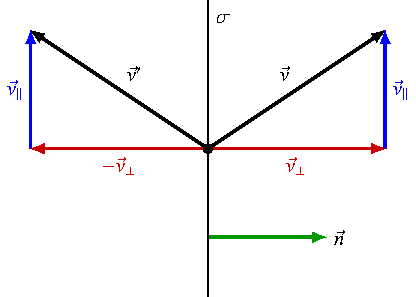
\includegraphics{4/images/spiegelung.pdf}
\end{center}
\caption{Spiegelung eines Vektors $\vec v$ an der Ebene senkrecht auf $\vec n$.
\label{image-spiegelung}}
\end{figure}
Da man mit dem Skalarprodukt senkrechte Projektionen berechnen kann,
muss es auch möglich sein, die Spiegelung eines Vektors $\vec v$
an einer Ebene mit Normale $\vec n$ zu berechnen ($|\vec n|=1$).
Dazu zerlegt man den Vektor $\vec v$ in eine Komponente $\vec v_{\|}$
parallel zur Ebene und eine Komponenten $\vec v_{\perp}$ senkrecht dazu,
also $\vec v=\vec v_{\|}+\vec v_{\perp}$ (Abbildung~\ref{image-spiegelung}).
Die senkrechte Komponente
ist im wesentlichen die Projektion von $\vec v$ auf $\vec n$:
\[
\vec v_{\perp}=
(\vec v\cdot\vec n)\vec n
.
\]
Die parallele Komponente ist der Rest:
\[
\vec v_{\|}=\vec v -\vec v_{\perp}=
\vec v-(\vec v\cdot\vec n)\vec n
,
\]
Beim gespiegelten Vektor zeigt die senkrechte Komponente in die
entgegengesetzte Richtung:
\begin{equation}
\vec v_{\text{gespiegelt}}=
\vec v_{\|}-\vec v_{\perp}
=
\vec v-(\vec v\cdot\vec n)\vec n
-
(\vec v\cdot\vec n)\vec n
=\vec v-2(\vec v\cdot\vec n)\vec n.
\label{equation:spiegelung}
\end{equation}

\begin{beispiel}
Man spiegle den Vektor $\vec a$ an der Ebene mit der Normalen $\vec n$,
\[
\vec a=\begin{pmatrix}1\\2\\3\end{pmatrix},
\qquad
\vec n=\begin{pmatrix}1\\1\\1\end{pmatrix}
\]

\smallskip

{\parindent 0pt Zunächst stellen wir fest,} dass $\vec n$ noch
kein Einheitsvektor ist, dass wir stattdessen $\vec n_0=\vec n/\sqrt{3}$
verwenden müssen.
Damit kann $\vec a$ jetzt die parallelen und orthogonalen
Komponenten zerlegt werden:
\[
\vec a_{\perp}=(\vec a\cdot\vec n_0)\vec n_0
=\frac1{\sqrt{3}} (1+2+3)\frac1{\sqrt{3}}\begin{pmatrix}1\\1\\1\end{pmatrix}
=\begin{pmatrix}2\\2\\2\end{pmatrix},
\quad
\vec a_{\|}=\begin{pmatrix} -1\\0\\1 \end{pmatrix}.
\]
Nach Formel (\ref{equation:spiegelung}) ist
\[
\vec a'=\vec a_{\|}-\vec a_{\perp}
=
\begin{pmatrix}-1\\0\\1\end{pmatrix}-\begin{pmatrix}2\\2\\2\end{pmatrix}
=\begin{pmatrix}-3\\-2\\-1\end{pmatrix}.
\]
der gespiegelt Vektor.
\end{beispiel}

